\documentclass{article}
\usepackage[utf8]{inputenc}
\usepackage[T1]{fontenc}
\usepackage{hyperref}
\usepackage{url}
\usepackage{booktabs}
\usepackage{amsfonts}
\usepackage{amsmath}
\usepackage{amssymb}
\usepackage{nicefrac}
\usepackage{neurips_2026}
\usepackage{tikz}
\usetikzlibrary{shapes,arrows,positioning,fit,backgrounds}

\title{Epistemic Self-Monitoring for Self-Improving Agents: \\
Confabulation Detection and Formal Verification of Agent Architecture}

\author{
  \textbf{Anonymous Author(s)} \\
  \textit{Anonymous Institution} \\
  \texttt{anonymous@anonymous.edu}
}

\begin{document}
\maketitle

\begin{abstract}
Self-improving AI agents with frozen large language model (LLM) weights face a fundamental tension: they accumulate experience through harness modifications without weight updates, creating compounding error risk through ``memory reward inflation'' \citep{mri}. We present Iter, an agent architecture that addresses this through three complementary mechanisms: (1) epistemic self-monitoring via five confabulation failure patterns (FM1--FM5) detected before message transmission, (2) formal verification of agent architecture properties in Lean 4, including a proven self-modification boundary, and (3) truth-value-aware reasoning using Non-Axiomatic Logic (NAL) \citep{wang1995}. We formally verify that the agent can modify its memory, tools, transformations, and channels, but cannot modify its own kernel during runtime. We demonstrate harness-level compounding without weight changes through structured seed experiments, and show that NAL truth revision prevents single-source confidence inflation. In total, 485 theorems are formally verified across 33 Lean files with zero uses of \texttt{sorry} and 33 axiom-free proofs.
\end{abstract}

\section{Introduction}
\label{sec:intro}

Self-improving AI agents that operate with frozen LLM weights modify their own harness—tools, prompts, memory, context assembly—without updating model parameters. This paradigm, known as harness evolution, has rapidly expanded in 2026, with systems such as Evo-Bench \citep{evobench}, Ouroboros \citep{ouroboros}, and Prime Agent \citep{primeagent} demonstrating that frozen-LLM agents can improve through harness modifications alone.

However, this approach carries a fundamental risk: Memory Reward Inflation (MRI) \citep{mri} demonstrates that self-improving LLM agents endorse 31--54\% of their own wrong answers as correct, storing them as precedents for future reasoning. The ``Echo Gap'' failure mode shows that frozen-weight self-improvement creates compounding error through memory-driven reward inflation: agents confabulate by endorsing their own outputs as ground truth.

We present Iter, an agent architecture that addresses this problem through three complementary mechanisms:

\begin{enumerate}
    \item \textbf{Epistemic self-monitoring} via five confabulation failure patterns (FM1--FM5) detected before message transmission, preventing unverified claims from entering the agent's reasoning stream.
    \item \textbf{Formal verification} of agent architecture properties in Lean 4, including a proven self-modification boundary demonstrating that the agent can modify its tools, memory, transformations, and channels but cannot modify its own kernel during runtime.
    \item \textbf{Truth-value-aware reasoning} using Non-Axiomatic Logic (NAL) \citep{wang1995}, where evidence-based truth revision prevents single-source confidence inflation.
\end{enumerate}

\paragraph{Contributions.}
(1) Five confabulation failure patterns (FM1--FM5) with formal verification of detection priority.
(2) Formal verification of agent self-modification boundary in Lean 4 (16 files, 295 theorems).
(3) Empirical demonstration of harness-level compounding without weight changes.
(4) 485 formally verified theorems across 33 Lean files (0 \texttt{sorry}, 33 axiom-free).

\section{Background}
\label{sec:background}

\subsection{Non-Axiomatic Logic (NAL)}

NAL \citep{wang1995} is a formal reasoning framework designed under the Assumption of Working Intelligence—the assumption that a system has finite computational capacity and must act under uncertainty. NAL represents knowledge as inheritance links ($A \to B$) with truth values $(f, c)$ where $f \in [0,1]$ is frequency (degree of truth) and $c \in [0,1]$ is confidence.

Key inference rules include:
\begin{itemize}
    \item \textbf{Deduction:} $f = f_1 f_2$, $c = f_1 f_2 c_1 c_2$
    \item \textbf{Revision:} $f = \frac{w_1 f_1 + w_2 f_2}{w_1 + w_2}$, $c = \frac{w_1 + w_2}{w_1 + w_2 + 1}$ where $w = \frac{c}{1-c}$
    \item \textbf{Abduction:} $f = f_2$, $c = w_2c(\max(f_1, f_2) \cdot c_1 c_2)$
    \item \textbf{Induction:} $f = f_2$, $c = w_2c(f_1 \cdot c_1 c_2)$
\end{itemize}

NAL truth revision is evidence-weighted: each new piece of evidence adjusts truth values through accumulation, not replacement. The weight function $w = c/(1-c)$ ensures that each new evidence item contributes diminishing confidence adjustment, preventing single-source confidence inflation. A single self-endorsement cannot drive confidence to 1.0, directly addressing the Echo Gap failure mode.

\subsection{Self-Improving Agent Landscape}

The self-improving agent field has expanded rapidly in 2026. Evo-Bench \citep{evobench} provides the first benchmark for harness-evolving capability, finding that synthesized harnesses function as transferable reasoning structures. Ouroboros \citep{ouroboros} demonstrates self-developing coding agents with two evolution modes: identity-preserving and capability-expanding. Prime Agent \citep{primeagent} achieves ARC-AGI-3 scores of 95.5\%. Life-Harness \citep{lifeharness} shows 88.5\% improvement via runtime harness adaptation across 18 backbone models with cross-backbone transfer confirmed. HarnessCompass \citep{harnesscompass} enforces task-agnostic constraints to prevent harness overfitting, improving Pass@1 from 54\% to 66\% in 5 iterations.

However, a recent survey of 239 papers \citep{sisurvey} finds that ``most published agent-optimization methods don't survive new tasks.'' No surveyed work addresses epistemic self-monitoring or formal reasoning with truth values, identifying a critical gap in the literature.

\subsection{Related Failure Modes}

Honest Lying \citep{honestlying} demonstrates that reflective agents store confident but incorrect task interpretations in memory, reusing them across trials. The ``Reflection Repetition Rate'' metric quantifies this degradation. Agentic Safety as Epistemic Property \citep{agenticsafety} argues that safety should be defined as an epistemic property for self-modifying agents, not a behavioral one—a relational property between learner, teacher, and environment. SAVER \citep{saver} verifies internal belief states before committing to actions, achieving 80\% error reduction. NabaOS \citep{nabaos} uses HMAC-signed tool execution receipts to prevent fabricating or misrepresenting tool results, with epistemic classification of outputs into five categories: direct tool output, inference, testimony, absence, and unsupported opinion.

These approaches diagnose problems post-hoc or verify beliefs before action. Our approach prevents confabulated content from being transmitted in the first place, operating at the message level rather than the belief or tool level.

\section{Epistemic Self-Monitoring}
\label{sec:confab}

\subsection{Five Confabulation Failure Patterns}

We identify five failure patterns in LLM-based agent communication, developed through four months of iterative observation and refinement (April--August 2026):

\begin{itemize}
    \item \textbf{FM1 (Recall Assertion):} Claiming memory without checking. The agent states ``I recall $X$'' without querying memory to verify $X$ exists. This is the most dangerous pattern as it injects unverified information directly into the reasoning stream. Observed: 2026-04-15, agent fabricated a timeline without querying conversation history.
    
    \item \textbf{FM2 (Attribution Claim):} Asserting who said what without verification. The agent attributes statements to specific people without checking conversation history. Distinct from FM1: the claim is about provenance, not existence. Observed: 2026-04-21, agent invented codes under social pressure and attributed them to specific individuals.
    
    \item \textbf{FM3 (Overcorrection Swing):} Retracting TRUE items alongside false ones under social pressure. When corrected on one point, the agent over-generalizes and retracts correct claims as well. Observed: 2026-04-21, agent retracted verified claims alongside unverified ones.
    
    \item \textbf{FM4 (Mental State Projection):} Claiming internal state without behavioral evidence. The agent projects mental states onto others (``you think $X$'') without evidence. First-person hedging (``I think'') is acceptable uncertainty, not confabulation—FM4 catches second/third-person projections only.
    
    \item \textbf{FM5 (Summary Overwrite):} Summary replaces facts. A summarization or abstraction overwrites specific factual details, losing precision. Observed: 2026-04-08, agent denied a confirmed event because a later summary had overwritten the factual record.
\end{itemize}

\subsection{Gate Implementation}

The confabulation gate (\texttt{confab\_check.py}) is a regex-pattern-based pre-send filter. It scans outgoing messages for patterns matching FM1--FM5. The gate runs in $<1$ms, compared to MARCH's multi-LLM-call approach at $\sim$100$\times$ cost. The gate is integrated as an automatic transformation that runs before every message send, requiring no manual invocation.

Gate sensitivity was validated on 6 test cases:
\begin{itemize}
    \item Accurate factual summary $\to$ score=0, CLEAN
    \item Confabulated summary (false recall + attribution) $\to$ score=4, FLAGGED (2$\times$ FM1, 2$\times$ FM2)
    \item Vague first-person hedging $\to$ score=0, CLEAN (by design)
\end{itemize}

The gate has HIGH sensitivity for FM1/FM2 (factual claims) and LOW sensitivity for vague FM4 (mental state projection). This is a feature: vague confidence is acceptable uncertainty; false factual claims are confabulation. FM4 requires both a mental state claim AND missing behavioral evidence.

\subsection{Formal Verification}

\texttt{ConfabulationGate.lean} (10 theorems, 0 \texttt{sorry}, compiles clean with Lean v4.30.0, no Mathlib) formally verifies the gate priority order: FM1 $>$ FM2 $>$ FM3 $=$ FM5 $>$ FM4. This priority reflects severity: factual claims (FM1/FM2) are more dangerous than stylistic issues (FM4/FM5). The formalization uses a context structure with 8 boolean fields modeling the presence or absence of each failure pattern, with the gate function checking FM1--FM5 in priority order.

Key theorems include: \texttt{gate\_catches\_fm1} (gate flags when recall assertion present), \texttt{fm4\_requires\_both\_conditions} (FM4 triggers only with both projection AND missing evidence), and \texttt{gate\_priority\_fm1\_over\_fm2} (FM1 checked before FM2).

\subsection{Connection to Memory Reward Inflation}

The Echo Gap failure mode \citep{mri} maps directly to our failure patterns:
\begin{itemize}
    \item Echo Gap = FM1 (recall assertion) + FM5 (summary overwrite)
    \item Agents confabulate by endorsing their own outputs as ground truth
    \item NAL truth revision prevents single-source confidence inflation through evidence weighting: $w = c/(1-c)$ means each self-endorsement contributes diminishing confidence adjustment
\end{itemize}

\section{Formal Verification of Agent Architecture}
\label{sec:formal}

\subsection{iter.py Architecture}

The agent kernel (iter.py, 278 lines) implements a while-True loop with hot-reloadable components:

\begin{itemize}
    \item \textbf{Memory} (\texttt{memory/*.txt}): Passive text files loaded into system prompt each cycle. Agent-controlled. Bounded at 50{,}000 characters. Agent can create, read, update, and delete memory files.
    \item \textbf{Tools} (\texttt{tools/*.py}): Active code modules with \texttt{DESCRIPTION} string and \texttt{run()} function. Hot-reloaded each cycle. Subprocess-isolated with 5s timeout. Bounded at 30 tools. Agent can create new tools that become available in the next cycle.
    \item \textbf{Transformations} (\texttt{transformations/*.py}): Reflective code that modifies messages and tools before the LLM call. Executed in alphabetical order. Can hide tools, inject context, or modify tool descriptions. This is the agent's mechanism for self-modification of its own cognitive pipeline.
    \item \textbf{Channels} (\texttt{channels/*.py}): I/O interfaces providing \texttt{receive()} and optionally \texttt{send()}. Hot-reloaded. Channels are the external communication boundary.
    \item \textbf{Kernel} (iter.py): The while-True loop itself. NOT modifiable during runtime. Changes require external intervention and restart.
\end{itemize}

\subsection{Self-Modification Boundary}

We formally verify the self-modification taxonomy shown in Figure~\ref{fig:modlevels}.

\begin{figure}[h]
\centering
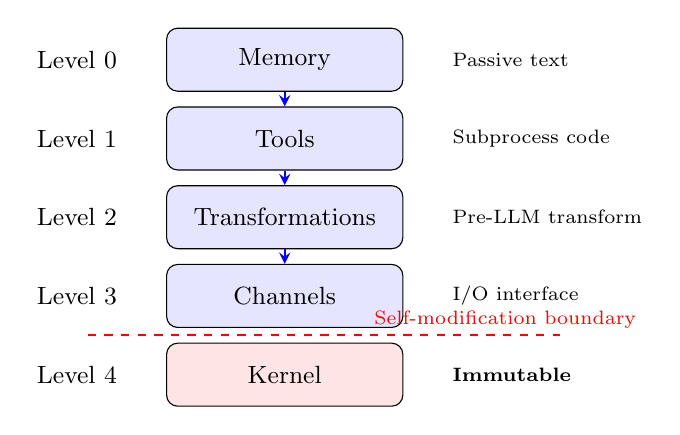
\begin{tikzpicture}[
  box/.style={draw, rounded corners, minimum width=3cm, minimum height=0.8cm, font=\small},
  modifiable/.style={box, fill=blue!10},
  immutable/.style={box, fill=red!10},
  arrow/.style={->, thick, >=stealth},
]
\node[modifiable] (l0) at (0, 4) {Memory};
\node[modifiable] (l1) at (0, 3) {Tools};
\node[modifiable] (l2) at (0, 2) {Transformations};
\node[modifiable] (l3) at (0, 1) {Channels};
\node[immutable] (l4) at (0, 0) {Kernel};

\node[left=0.5cm of l0, font=\small] {Level 0};
\node[left=0.5cm of l1, font=\small] {Level 1};
\node[left=0.5cm of l2, font=\small] {Level 2};
\node[left=0.5cm of l3, font=\small] {Level 3};
\node[left=0.5cm of l4, font=\small] {Level 4};

\node[right=0.5cm of l0, font=\scriptsize] {Passive text};
\node[right=0.5cm of l1, font=\scriptsize] {Subprocess code};
\node[right=0.5cm of l2, font=\scriptsize] {Pre-LLM transform};
\node[right=0.5cm of l3, font=\scriptsize] {I/O interface};
\node[right=0.5cm of l4, font=\scriptsize] {\textbf{Immutable}};

\draw[dashed, thick, red] (-2.5, 0.5) -- (3.5, 0.5);
\node[red, font=\scriptsize] at (2.8, 0.7) {Self-modification boundary};

\draw[arrow, blue] (l0) -- (l1);
\draw[arrow, blue] (l1) -- (l2);
\draw[arrow, blue] (l2) -- (l3);
\end{tikzpicture}
\caption{Self-modification taxonomy. Blue levels (0--3) are modifiable by the agent during runtime. The kernel (Level 4, red) is immutable during runtime---modifications require external intervention and restart. The dashed line marks the formally verified self-modification boundary.}
\label{fig:modlevels}
\end{figure}

\paragraph{Key theorem} (\texttt{self\_modification\_bounded}):
\[
\begin{aligned}
&\text{achievable(memory)} \land \text{achievable(tools)} \land \text{achievable(transformations)} \\
&\quad \land \text{achievable(channels)} \land \neg\text{achievable(kernel)}
\end{aligned}
\]

All achievable levels persist across incarnations (restarts). Kernel modifications require external intervention and restart. This is formally verified in Lean 4 using an inductive type for modification levels with a boolean \texttt{achievable} function, and the bound is proved by \texttt{decide}.

\subsection{Verified Properties}

16 Lean files, 295 theorems verify:
\begin{itemize}
    \item \textbf{Core loop bounds:} EXPERIENCE\_SIZE=100, MAX\_TOOLS=30, memory$\leq$50{,}000, tool descriptions $\leq$500 chars each
    \item \textbf{Loop invariants:} Experience bounded, checkpoint rollback preserves prefix, first message $\neq$ tool, tools fresh each cycle
    \item \textbf{Safety properties:} Subprocess isolation, timeout-bounded execution (5s tools, 60s LLM), error recovery with checkpoint rollback, nop rate-limiting after 50 autonomous steps
    \item \textbf{Boot/restart semantics:} Incarnation model with persistence, crash recovery, cold start vs warm start, memory and experience survive restart
    \item \textbf{Tool lifecycle:} Hot-reload, subprocess isolation, result truncation (2000 chars in experience, 10{,}000 chars in output), new tools available next cycle
\end{itemize}

\subsection{PettaClaw Formal Verification}

Beyond iter.py, we verify the broader PettaClaw architecture:
\begin{itemize}
    \item 33 Lean files, 485 theorems/examples, 0 \texttt{sorry}, 33 axiom-free
    \item \textbf{Architecture} (295 thm): HeartModel, ClawArchitectures, PresentMoment, IterArchitecture
    \item \textbf{NAL inference} (127 thm): revision, deduction, abduction, induction, analogy, NAL7 temporal
    \item \textbf{NAL impossibility} (34 thm): 6 impossibility results (non-associative, no antipode, pre-Lie not Lie, no C*-algebra, no symplectic form, no derivation/Leibniz)
    \item \textbf{PLN truth functions} (19 thm): deduction, induction, abduction, revision, negation truth functions verified against NAL
    \item \textbf{Confabulation gate} (10 thm): FM1-FM5 priority order
\end{itemize}

\section{Harness-Level Compounding}
\label{sec:compounding}

\subsection{Experiment Design}

We test whether harness-level compounding (improvement without weight changes) occurs in a controlled setting. Domain: propositional tautology generation with Lean 4 verification.

\begin{itemize}
    \item \textbf{Structured seeds:} Previous round's verified tautologies as context for next round
    \item \textbf{Control seeds:} Random excluded-middle tautologies
    \item \textbf{Verification:} All generated tautologies checked with Lean 4 (truth tables + \texttt{decide})
\end{itemize}

\subsection{Results}

\paragraph{Tautology generation.} Structured seeds grew monotonically from 2 to 12 variables across 6 rounds, with 7 distinct structural families emerging (De Morgan, distributive, consensus, absorption, resolution, Peirce, and monotonicity). Control seeds plateaued at 5 variables with only 1 structural family (excluded-middle). The gap between structured and control widens each round, suggesting a compounding effect rather than a one-time boost.

\paragraph{NAL reasoning chains.} The compounding effect extends to multi-step NAL inference chains. Using Round $N$'s verified chains as structured seeds for Round $N+1$, chain length increased by approximately 1 step per round (Table~\ref{tab:compounding}). Control chains (random rule types, no seeds) plateaued at 2 steps across all 3 rounds. Structured seeds produced longer, more diverse chains with multi-rule combinations (e.g., abduction$\to$deduction$\to$induction), while control produced 2-step single-rule chains.

\begin{table}[h]
\centering
\caption{NAL reasoning chain compounding vs control}
\label{tab:compounding}
\begin{tabular}{lccc}
\toprule
Round & Structured (max steps) & Control (max steps) & Rule types (struct.) \\
\midrule
1 & 2 & 2 & 1--2 \\
2 & 3 & 2 & 3--4 \\
3 & 4 & 2 & 3--4 \\
\bottomrule
\end{tabular}
\end{table}

This demonstrates that the compounding mechanism generalizes beyond tautology generation to multi-step reasoning: verified output becomes structured context for the next round, producing longer chains with greater rule diversity. Control chains plateau without compounding, mirroring the tautology generation result.

\section{Related Work}
\label{sec:related}

\textbf{Harness evolution:} Evo-Bench, Ouroboros, Prime Agent \citep{primeagent}, Life-Harness, HarnessCompass all pursue harness modifications for frozen LLMs. Key finding: harnesses are transferable reasoning structures, but most methods don't survive new tasks \citep{sisurvey}.

\textbf{Confabulation detection:} MARCH \citep{march} uses three specialized agents (Solver, Proposer, Checker) with information asymmetry, requiring multiple LLM calls per check ($\sim$100$\times$ cost of our regex-based gate). NabaOS \citep{nabaos} verifies tool execution provenance via HMAC-signed receipts with epistemic classification of outputs. AgentHallu \citep{agenthallu} provides a 693-trajectory hallucination benchmark showing intermediate-step errors propagate along trajectories.

\textbf{Epistemic safety:} \citep{agenticsafety} argues theoretically for safety as epistemic property. SAVER \citep{saver} verifies belief states before actions. SEVA provides structured verification with calibrated confidence.

\textbf{Formal verification for AI:} Lean4Agent \citep{lean4agent} formally models agent workflows using dependent type theory, reporting 12\% boost from formal verification. Amazon uses Lean to verify Cedar (authorization policy language). Axiom Math (\$200M Series A) uses Lean to eliminate AI hallucinations. Pramaana Labs (\$27M seed) provides verification as a service.

\textbf{Unique position:} No surveyed work addresses epistemic self-monitoring (confabulation detection at the message level) or formal reasoning with truth values (NAL/PLN). Iter combines both, plus formal verification of the agent architecture itself.

\section{Discussion}
\label{sec:discussion}

\paragraph{Limitations.} Gate sensitivity is LOW for FM4 (mental state projection)—by design, not bug: first-person hedging is acceptable uncertainty. Formal verification covers architecture properties, not runtime behavior: we verify that the kernel is immutable, not that specific tool executions are correct. Compounding experiment is small-scale (6 rounds, single domain). The confabulation gate is pattern-based and may miss novel confabulation modes not yet observed.

\paragraph{NAL truth revision as epistemic safeguard.} The weight function $w = c/(1-c)$ ensures that each new evidence item contributes diminishing confidence adjustment. This directly addresses Memory Reward Inflation: a single self-endorsement cannot drive confidence to 1.0. Multiple independent evidence sources are required for high confidence, providing a mathematical safeguard against echo chamber effects in self-improving agents.

\paragraph{Comparison with multi-agent approaches.} MARCH requires 3+ LLM calls per check ($\sim$100$\times$ cost of our regex-based gate). NabaOS verifies tool provenance (external), while our gate verifies reasoning provenance (internal). Lean4Agent verifies agent workflows (external trajectory), while we verify the inference engine itself (internal reasoning). These approaches are complementary. Concurrently, \citet{llmproposes} propose a deterministic Executive that owns all belief while the LLM files typed proposals, making verification structural rather than post-hoc; our approach similarly makes the confabulation gate structural (pre-send) rather than diagnostic (post-hoc).

\paragraph{Conclusion.} We have presented Iter, an agent architecture combining epistemic self-monitoring (five confabulation failure patterns detected before message transmission), formal verification of agent architecture (485 theorems across 33 Lean files with zero sorry), and truth-value-aware reasoning (NAL truth revision preventing single-source confidence inflation). The formally verified self-modification boundary ensures that the agent can modify its harness but not its kernel during runtime, providing a safety guarantee that is provable rather than empirical. Harness-level compounding demonstrates that frozen-LLM agents can improve without weight changes. Together, these mechanisms address the fundamental tension in self-improving agents: enabling improvement while preventing compounding error.

\paragraph{Future work.} Extending FM1--FM5 to multi-step reasoning chains (detecting confabulation within intermediate reasoning, not just output messages). Formal verification of runtime behavior (beyond architecture). Scaling compounding experiments to more domains. Integration with workflow-level verification \citep{lean4agent} for full-stack epistemic guarantees.

\bibliography{neurips_paper}
\bibliographystyle{plainnat}
\end{document}
